\section{Graph Databases}

\AP ""Graph databases"" are abstracted as edge-labelled directed graphs
$G = \langle \vertex{G}, \edges{G} \rangle$, 
where nodes of $\intro*\vertex{G}$ represent entities and labelled edges $\intro*\edges{G} \subseteq \vertex G \times \A \times \vertex G$
represent relations between these entities, with $\A$ being a fixed finite alphabet.
For instance, \Cref{fig:example-graph-database} depicts a "graph database",
whose nodes are authors and papers, on the alphabet
$\A = \{\text{\color{wrote}wrote},\,\text{\color{advised}advised}\}$.
Edges $x \atom{\wrote} y$ indicate that the person $x$ wrote the paper $y$,
while edges $x \atom{\advised} y$ indicate that person $x$ was
the Ph.D. advisor of person $y$.

\begin{figure}[ht]
    \centering
    \begin{tikzpicture}
        \node (a1) {author$_1$};
        \node (a2) [right = of a1] {author$_2$};
        \node (a3) [right = of a2] {author$_3$};
        \node (a4) [right = of a3] {author$_4$};
        \node (a5) [right = of a4] {author$_5$};
        \node (p1) [below = 2.5em of a2] {paper$_1$};
        \node (p2) [below = 2.5em of a3] {paper$_2$};
        \node (p3) [below = 2.5em of a4] {paper$_3$};

        \draw[wrote] (a1) to[edge, ->] node[fill=white] {\footnotesize wrote} (p1)
            (a2) to[edge, ->] node[fill=white] {\footnotesize wrote} (p1)
            (a2) to[edge, ->] node[fill=white] {\footnotesize wrote} (p2)
            (a3) to[edge, ->] node[fill=white] {\footnotesize wrote} (p2)
            (a4) to[edge, ->] node[fill=white] {\footnotesize wrote} (p3)
            (a5) to[edge, ->] node[fill=white] {\footnotesize wrote} (p3);
        \draw[advised] (a4) to[edge, ->, bend right=60] node[fill=white] {\footnotesize advised} (a3)
            (a5) to[edge, ->, bend right=60] node[fill=white] {\footnotesize advised} (a4);
    \end{tikzpicture}
    \caption{%
        \AP\label{fig:example-graph-database}%
        A "graph database" with eight nodes and eight edges on a two-letter alphabet.
    }
\end{figure}

\AP Being a subclass of relational databases, "graph databases" can be queried by the
predominant query language of ""conjunctive queries"", "aka" "CQs", 
which consists of the closure under projection---"aka" existential quantification---of conjunctions of atoms of the form $x \atom{a} y$
for some letter $a \in \A$. For instance, the "conjunctive query"
\[
    \gamma_1(x, y) = x \atom{\wrote} z
        \land y \atom{\wrote} z    
\]
returns, when "evaluated" on the "graph database" $G$
defined in \Cref{fig:example-graph-database}, all pairs of nodes $(u, v)$ such that $u$ is a co-author
of $v$. Each variable not appearing in the left-hand side of 
the definition of a "conjunctive query" (in this example, $z$) is implicitly 
existentially quantified. 
Note that, to the cost of losing the information of which variable is existentially quantified, every "CQ"
can be seen as a "graph database", where each variable is a node, and each atom is an edge; 
hence, we sometimes use "graph database" terminology for "CQs".

The expressive power of "CQs" is somewhat limited, since
"CQs" cannot express, for example, transitive closure.
Since the ability to navigate paths is of importance in many "graph database" 
scenarios, most modern graph query languages support, as a central querying mechanism,
"conjunctive regular path queries", or "CRPQs" for short. 
In particular, "CRPQs" form the core navigational mechanism of the new ISO standard Graph Query Language (GQL) \cite{ISO2024GQL} and the SQL extension for querying graph-structured data SQL/PGQ \cite{ISO2023PGQ} (see also \cite{FrancisEtal2023GQL,FrancisEtal2023GPC}).

"CRPQs" are 
defined analogously to "conjunctive queries", except that their atoms are now of the form 
$x \atom{L} y$ where $L$ is an arbitrary regular language over the alphabet $\A$. For 
instance the "evaluation" of the "CRPQ"
\[
    \gamma_2(x, y) = x \atom{\wrote} z
        \land z' \atom{\wrote} z 
        \land y \atom{({\advised})^*} z'
\]
on $G$ yields every pair of persons $(u,v)$ such that $u$ is a co-author of a
``scientific descendant'' of $v$. 

\AP Formally, a ""CRPQ"" $\gamma$ is defined as a tuple $\bar z = (z_1,\hdots,z_n)$
of ""output variables"", "aka" \reintro{free variables},\footnote{For technical reasons (see the definition of "equality atoms") we allow for a variable to appear multiple times.}
together with a conjunction of ""atoms"" of the form
$\bigwedge_{j=1}^m x_j \atom{L_j} y_j$, where each $L_j$ is a regular language and where $m \geq 0$.
The set of all variables occurring in $\gamma$, namely\footnote{We neither assume 
disjointness nor inclusion between $\{z_1,\hdots,z_n\}$ and $\{x_1,y_1,\hdots,x_m,y_m\}$}
$\{z_1,\hdots,z_n\}\cup\{x_1,y_1,\hdots,x_m,y_m\}$, is denoted by
$\intro*\vars(\gamma)$.
Given a "database@@graph" $G$, we say that a tuple of nodes $\bar u = (u_1,\hdots,u_n)$
\AP""satisfies@@db"" $\gamma$ 
on $G$ if there is a mapping
$\fun\colon \vars(\gamma) \to \vertex{G}$ such that $u_i = \fun(z_i)$ for all
$1 \leq i \leq n$, and for each $1 \leq j \leq m$,
there exists a path from $\fun(x_i)$ to $\fun(y_i)$ in $G$, labelled by
a word from $L_i$ (if the path is empty, the label is $\epsilon$). The \AP""evaluation"" of $\gamma$ on $G$ is then the set of all tuples that "satisfy@@db" $\gamma$.
%
For example, $(\text{author}_2, \text{author}_5)$ "satisfies@@db" $\gamma_2$ 
on the "graph database" $G$ of \Cref{fig:example-graph-database} via
the function that maps $x$ to $\text{author}_2$, $y$ to $\text{author}_5$,
$z$ to $\text{paper}_2$, and $z'$ to $\text{author}_3$.

\AP
The language of "CRPQ" can be extended to navigate edges in both directions. 
\knowledgenewrobustcmd{\Gpm}{\cmdkl{G^\pm}}
Consider the expanded database $\intro*\Gpm$ obtained from $G$ by 
% keeping the same vertices, copying the edges of $G$, and 
adding, for every edge $x \atom{a} y$ in $G$, an extra edge $y \atom{a^-} x$.
We obtain a graph database on the alphabet $\intro*\Aext = \A \cup \A^-$ where
$\A^- = \set{a^- \mid a \in \A}$. We then define the syntax of
a \AP""CRPQ with two-way navigation"", or \reintro{C2RPQ}, as a "CRPQ" on the alphabet $\Aext$.
Its \reintro{evaluation} is defined as the "evaluation" of the "CRPQ" on $\Gpm$.
For instance, the "evaluation" of the "C2RPQ"
\[
    \gamma_3(x, y) = x \atom{({\wrote}\cdot{\wrote}^-)^*} y
\]
on the "graph database" of \Cref{fig:example-graph-database} returns all pairs of
individuals linked by a chain of co-authorship.
It includes $(\text{author}_1, \text{author}_3)$ or $(\text{author}_1, \text{author}_1)$
but not $(\text{author}_1, \text{author}_4)$.
%
\AP If a query has no "output variables" we call it ""Boolean"", and
its "evaluation" can either be the set $\set{()}$, in which case we say that $G$
\reintro(db){satisfies} the query, or the empty set $\set{}$. For example, $G$ "satisfies@@db" the
"Boolean CRPQ"
\[\gamma_4() = x \atom{\wrote} y\]
if, and only if, the database contains one author together with one paper they wrote.

We denote the set of "atoms" of a "C2RPQ" $\gamma$ by \AP$\intro*\atoms\gamma$, and by 
$\intro*\nbatoms{\gamma}$ we denote its number of "atoms", "ie", $|\atoms\gamma|$.
Moreover, we denote by $\intro*\size{\gamma}$ the sum of its number of "atoms" with
the sum of the size of NFAs used to describe $\gamma$.

\AP Finally, a ""union of CQs"" (\reintro{UCQs}) (resp.\ ""union of CRPQs"" (\reintro{UCRPQs}), resp.\ ""union of C2RPQs"" (\reintro{UC2RPQs}))  
is defined as a finite set of "CQs" (resp.\ "CRPQs", resp.\ "C2RPQs"), whose
tuples of "output variables" have all the same arity. 
\AP
A ""subquery"" of a "C2RPQ" $\gamma$ is any "C2RPQ" resulting from removing some "atoms" (possibly none) from $\gamma$. A \reintro{subquery} of  "UC2RPQ" is a union of "subqueries" of the "C2RPQs" therein.
The "evaluation" of a union is defined as the union of its "evaluations", for instance the following "UCQ"
\begin{align*}
    \Gamma_5 & = \gamma_{5}^1(x, y) \lor \gamma_{5}^2(x, y) \\
    & \text{ where }
    \gamma_{5}^1(x, y) = x \atom{\wrote} y %\\
    \text{ and }
    \gamma_{5}^2(x, y) = x \coatom{\advised} z \land
        z \atom{\wrote} y
\end{align*}
"evaluates" to the set of pairs $(x,y)$ such that $y$ is a paper written by either $x$
or their advisor.
We naturally extend the notations $\nbatoms{-}$ and $\size{-}$ to "unions@UC2RPQs".
\AP ""Infinitary unions"" are defined analogously, except
that we allow for potentially infinite unions. We often use a set notation to denote the union, especially for "infinitary unions".

For a more detailed introduction to "CRPQs", we refer the reader to \cite{Figueira2020Containment21Foundations}.
For a more general introduction to different query languages for "graph databases"---including "CRPQs"---see \cite{Barcelo2013Querying}, and for a more practical approach,
see \cite{AnglesEtal2017Foundations}.

\smallskip

% \paragraph*{Containement and equivalence}
\AP %It is often interesting to compare queries together. 
The ""evaluation problem"" for "UC2RPQ" is the problem of, given
a "UC2RPQ" $\Gamma$, a "graph database" $G$ and a tuple $\bar u$ of elements of $G$,
whether $\bar u$ "satisfies@@db" $\Gamma$ on $G$. 
Given two "UC2RPQ" $\Gamma$
and $\Gamma'$ whose "output variables" have the same arity,
we say that $\Gamma$ is \AP""contained"" in $\Gamma'$,
denoted by $\Gamma \intro*\contained \Gamma'$ if
for every "graph database" $G$, for every tuple $\bar u$ of $G$,
if $\bar u$ "satisfies@@db" $\Gamma$ on $G$, then so does $\Gamma'$ (we will hence reserve the symbol `$\subseteq$' for set inclusion---note in particular that inclusion (of the "UC2RPQs", seen as sets of "C2RPQs") implies "containment", but the converse does not hold). 
The \AP""containment problem"" for "UC2RPQs" is the problem of, given
two "UC2RPQs" $\Gamma$ and $\Gamma'$, to decide if $\Gamma \contained \Gamma'$.
When $\Gamma$ is "contained" in $\Gamma'$ and vice versa, we say that
$\Gamma$ and $\Gamma'$ are \AP""semantically equivalent"", denoted by
$\Gamma \intro*\semequiv \Gamma'$. 

\begin{itemize}
	\itemAP $\intro*\Exp$ and ""expansion""
	\itemAP $\intro*\cdb$ and ""canonical database""
	\itemAP $\intro*\Refin$, ""atom refinement"", ""refinement""
	\itemAP $\intro*\contract{L_i \cdots L_{j}}$, ""one-way contraction"", ""contraction"" and ""condensation"" -> unify terminology; ""contracting internal variables"", ""internal path""
	\itemAP $\intro*\nbatoms{\gamma}$, $\intro*\nbvar{\gamma}$
	\itemAP ""evaluation map""
	\itemAP ""simple regular expression"" and ""positive simple regular expression""
\end{itemize}

A \AP""class of (Boolean) CRPQs"" is a function \AP$\intro*\classCRPQ$ mapping an alphabet $\A$ 
to a set $\classCRPQ_{\A}$ of "Boolean CRPQs", which is closed under variable renaming and alphabetic
renaming of the languages.

The \reintro{tree-width} of a "C2RPQ" is the "tree-width" of its underlying multigraph. 
We denote by $\intro*\Tw$ (resp.\ $\intro*\TwOneWay$) the set of all "C2RPQs" (resp.\ "CRPQs") of "tree-width" at most $k$. The \reintro{tree-width} of a "UC2RPQ" is simply the maximum of the "tree-width" of its "C2RPQs".
\AP The \reintro{path-width} of a "C2RPQ" and "UC2RPQ" are defined analogously. We denote by \AP$\intro*\Pw$ (resp.\ $\intro*\PwOneWay$) the set of all "C2RPQs" (resp.\ "CRPQs") of "path-width" at most $k$. The relationship between these classes is depicted in \Cref{fig:taxonomy-syntactic}:
note that $\TwOneWay$ and $\PwOneWay$ are not explicitly drawn, but correspond to the
intersection of $\Tw$ (resp.\ $\Pw$) with the class of "CRPQs".

\begin{figure}
	\centering
	\scalebox{1.125}{
	\begin{tikzpicture}
		\node at (0,0) {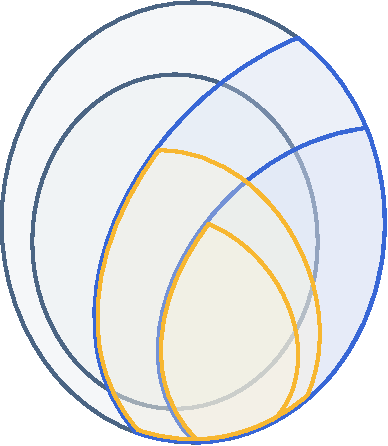
\includegraphics[scale=.8]{fig/semantic-tw/taxonomy-syntactic.pdf}};
		% \draw[line width=1.5pt] (0,-4) -- (0,4);
		% \draw[line width=1.5pt] (-3,0) -- (3,0);
		% \draw[line width=.5pt] (1,-4) -- (1,4);
		% \draw[line width=.5pt] (-3,1) -- (3,1);
		% \draw[line width=.5pt] (-1,-4) -- (-1,4);
		% \draw[line width=.5pt] (-3,-1) -- (3,-1);
		\node[font=\small] at (.5,-1.5)
			{$\withkl{\kl[\Pw]}{\cmdkl{\color{cYellow}\mathcal{P\hspace{-.15em}w}_{1\!}}}$};
		\node[font=\small] at (-.5,0) 
			{$\withkl{\kl[\Pw]}{\cmdkl{\color{cYellow}\mathcal{P\hspace{-.15em}w}_{k\!}}}$};
		\node[font=\small] at (2.05,.2)
			{$\withkl{\kl[\Tw]}{\cmdkl{\color{cBlue}\mathcal{T\hspace{-.15em}w}_{1\!}}}$};
		\node[font=\small] at (1.4,1.8)
			{$\withkl{\kl[\Tw]}{\cmdkl{\color{cBlue}\mathcal{T\hspace{-.15em}w}_{k\!}}}$};
		\node[font=\tiny] at (-1.5,.5) {\kl[CRPQ]{\color{cDarkGrey}CRPQs}};
		\node[font=\tiny] at (-.5,2.4) {\kl[C2RPQ]{\color{cDarkGrey}C2RPQs}};
	\end{tikzpicture}
	}
	\caption{
		\AP\label{fig:taxonomy-syntactic}
		Clickable taxonomy of syntactic classes defined using "tree-width".
	}
\end{figure}


Similar statements of the following proposition can be considered Folklore (see "eg" {\cite[Theorem IV.3]{RomeroBarceloVardi2017Homomorphism}}); however, our inability to find a proof for it with sharp bounds invites us to include a proof.
\begin{restatable}[Proof in \Cref{apdx-sec:prop:crpq-bound-tree-width-upper-bound}]{proposition}{crpqboundtwupperbound}
	\AP\label{prop:crpq-bound-tree-width-upper-bound}
    For each $k \geq 1$, the "evaluation problem" for "UC2RPQs" of "tree-width" at
    most $k$ can be solved in time $\+O(\size{\Gamma} \cdot |G|^{k+1} \cdot \log{|G|})$ on a Turing machine,
	or $\+O(\size{\Gamma} \cdot |G|^{k+1})$ under a RAM model, where $\Gamma$ and $G$ are the input "UC2RPQ" and "graph database", respectively.
\end{restatable}

In practice, "graph databases" tend to be huge and often changing, while queries
are in comparison very small.
This motivates the following question, given some natural $k \geq 1$: 

\begin{center}
    \AP 
    Given a "UC2RPQ" $\Gamma$, is it "equivalent" to a "UC2RPQ" $\Gamma'$ of "tree-width" at most $k$?\\
    That is, does it have ""semantic tree-width"" at most $k$?
\end{center}
This problem is called the ""semantic tree-width $k$ problem"".
Should it be decidable in a constructive way---that is, decidable, and if the answer is positive, we can compute a witnessing $\Gamma'$ from $\Gamma$---, then one could, once and for all,
compute $\Gamma'$ from $\Gamma$ and, whenever one wants to "evaluate" $\Gamma$ on a
database, "evaluate" $\Gamma'$ instead.

We will also study the restriction of these notions to one-way queries: a "UCRPQ" has \AP""one-way semantic tree-width"" at most $k$ if it is equivalent to a "UCRPQ" of "tree-width" at most $k$. The \AP""one-way semantic tree-width $k$ problem"" is the problem of, given a "UCRPQ" $\Gamma$, whether it has "one-way semantic tree-width" at most $k$.

\begin{example}
    \AP\label{ex:CRPQ-tw3-stw2}
    Consider the following "CRPQs",\footnote{In this graphical representation,
	we interpret a labelled graph as the "CRPQ" defined as
	the conjunction of the "atoms" induced by the labelled edges of the graph.
	For instance, $\gamma(\bar x)$ is a conjunction of six "atoms".}
    where $\bar x = (x_0,x_1,y,z)$:\leavevmode
    \begin{center}
        \small
        \begin{tikzcd}[column sep=small, row sep=small]
            &[-.5em] x_0 \ar[dr, "a"] \ar[rr, "c"] \ar[ddr, "a(bb)^+" swap, pos=.6, bend right] & &
            x_1 \ar[dl, "a" swap] \ar[ddl, "ab(bb)^*", pos=.7, bend left]
                &[1.5em] &[-.5em] x_0 \ar[dr, "a"] \ar[rr, "c"] \ar[ddr, "a(bb)^+" swap, pos=.6, bend right] & &
                x_1 \ar[dl, "a" swap] 
                    &[1.5em] &[-.5em] x_0 \ar[dr, "a"] \ar[rr, "c"]  & &
                    x_1 \ar[dl, "a" swap] \ar[ddl, "ab(bb)^*", pos=.6, bend left] \\
            \gamma(\bar x) \defeq & & y \ar[d, "b^+", pos=.35] & 
                & \delta(\bar x) \defeq & & y \ar[d, "b(bb)^*" pos=.35] & 
                    & \delta'(\bar x) \defeq & & y \ar[d, "(bb)^+" swap, pos=.35] & \\
            & & z & 
                & & & z & 
                    & & & z &
        \end{tikzcd}
    \end{center}
    \noindent
    The underlying graph of $\gamma(\bar x)$ being the directed 4-clique, $\gamma 
    (\bar x)$ has "tree-width" 3. We claim that $\gamma(\bar x)$ is equivalent to the "UCRPQ"
    $\delta(\bar x) \lor \delta'(\bar x)$, and hence has "one-way semantic tree-width" at most 2.

    Indeed, given a "graph database" satisfying $\gamma(\bar x)$ via some mapping $\mu$, 
    it suffices to make a case disjunction on whether the number of $b$-labelled "atoms"
    in the path from
    $\mu(y)$ to $\mu(z)$ is even or odd. In the first case, the "atom" $x_0\atom{a(bb)^+} z$ becomes
    redundant since we can deduce the existence of such a path from the conjunction
    $x \atom{a} y \atom{(bb)^+} z$, and hence the "database@@graph" "satisfies@@db" $\delta(\bar x)$ via $\mu$.
    Symmetrically, in the second case, the "atom" $x_1 \atom{b(bb)^*} z$ becomes redundant,
    and the "database@@graph" "satisfies@@db" $\delta'(\bar x)$ via $\mu$. 
    Thus, $\gamma(\bar x)$
    is "contained", and hence "equivalent" (the other "containment" being trivial), to
    the "UCRPQ" $\delta(\bar x) \lor \delta'(\bar x)$ of "tree-width" 2.
\end{example}

\subsection{\AP{}Related Work}
\label{sec:relwork}
On the class "conjunctive queries", the "semantic tree-width $k$ problem" becomes the "coNP"-complete problem of finding out whether the retraction of a query has "tree-width"
at most $k$. In fact, "CQs" enjoy the effective existence of unique minimal queries \cite[Theorem 12]{ChandraMerlin1977Implementation}, which happen to also minimize the tree-width. For "CRPQs" and "UC2RPQs", the question is far more challenging, and it has only been solved for the case $k = 1$ 
by Barceló, Romero, and Vardi \cite[Theorem 6.1]{BarceloRomeroVardi2016SemanticAcyclicity}; the case $k>1$ was left widely open
\cite[\S 7]{BarceloRomeroVardi2016SemanticAcyclicity}.

Furthermore, classes of "CQs" of bounded "semantic tree-width" precisely characterize tractable (and "FPT") "evaluation problem" \cite[Theorem~1.1]{Grohe2007ComplexityHomomorphism}.
This result is on bounded-arity schemas, which was later generalized \cite[Theorem~1]{ChenGottlobLanzingerPichler2020Semantic} for characterizing "FPT" "evaluation" on arbitrary schemas---by replacing "semantic tree-width" with semantic ``submodular width'' \cite{Marx13Tractable}.

The problem of computing "maximal under-approximations" of "CQs" of a given "tree-width" has been explored in \cite{BarceloLibkinRomero2014Efficient}.
A "maximal under-approximations" of tree-width at most $k$ of a "CQ" $\gamma$ consists of a
"CQ" $\delta_k$ of "tree-width" at most $k$, which under-approximates it,
"ie" $\delta_k$ is "contained" in $\gamma$, and which is maximal, in the sense that for every "CQ" 
$\delta'$, if $\delta'$ has "tree-width" at most $k$ and is "contained" in $\gamma$, then 
$\delta'$ is "contained" in $\delta_k$. 
"Maximal under-approximations" of a given "tree-width" for "CQs" always exist \cite{BarceloLibkinRomero2014Efficient} and thus, a "CQ" is "semantically equivalent"
to a "CQ" of "tree-width" at most $k$ if, and only if, it is equivalent to its maximal under-approximation of "tree-width" at most $k$. Our solution to decide the
"semantic tree-width $k$ problem" for "UC2RPQs" is based on this idea.

While "maximal under-approximations" always exist for "CQs", this is not the case for the dual notion of ``minimal over-approximations''. The problem of when these exist is still unknown to be decidable, aside for some the special cases of acyclic "CQs" and Boolean "CQs" over binary schemas \cite{BarceloRomeroZeume2020Approximation}.

% % ---
% % Minimization paper
% % ---

% \paragraph{Graph databases.}
% \AP ""Graph databases"" are abstracted as edge-labelled directed graphs
% $G = \langle \vertex{G}, \edges{G} \rangle$, 
% where nodes of $\intro*\vertex{G}$ represent entities and labelled edges $\intro*\edges{G} \subseteq \vertex G \times \A \times \vertex G$
% represent relations between these entities, with $\A$ being a fixed finite alphabet.

% \paragraph{Conjunctive regular path queries (CRPQs) and unions of CRPQs (UCRPQs).}
% \AP A ""CRPQ"" $\gamma$ is defined as a tuple $\bar z = (z_1,\hdots,z_n)$
% of ""output variables""\footnote{For technical reasons (see the definition of "equality atoms") we allow for a variable to appear multiple times.},
% together with a conjunction of ""atoms"" of the form
% \AP$\bigwedge_{j=1}^m x_j \intro*\atom{L_j} y_j$, where each $L_j$ is a regular language
% and where $m \geq 0$.
% The set of all variables occurring in $\gamma$, namely%
% \footnote{We neither assume 
% disjointness nor inclusion between $\{z_1,\hdots,z_n\}$ and $\{x_1,y_1,\hdots,x_m,y_m\}$.}
% $\{z_1,\hdots,z_n\}\cup\{x_1,y_1,\hdots,x_m,y_m\}$, is denoted by
% $\intro*\vars(\gamma)$. Variables in $\vars(\gamma)\setminus \{z_1,\hdots,z_n\}$ are existentially quantified. 
% We denote by $\intro*\atoms(\gamma)$ the set of "atoms" of $\gamma$.
% Given a "database@@graph" $G$, we say that a tuple of nodes $\bar u = (u_1,\hdots,u_n)$
% \AP""satisfies@@db"" $\gamma$ 
% on $G$ if there is a mapping
% $\fun\colon \vars(\gamma) \to \vertex{G}$ such that $u_i = \fun(z_i)$ for all
% $1 \leq i \leq n$, and for each $1 \leq j \leq m$,
% there exists a (directed) path from $\fun(x_j)$ to $\fun(y_j)$ in $G$, labelled by
% a word from $L_j$ (if the path is empty, the label is $\varepsilon$). The \AP""evaluation"" of $\gamma$ on $G$ is then the set of all tuples that "satisfy@@db" $\gamma$ on $G$.

% A ""union of CRPQs"" (\reintro{UCRPQs})
% is defined as a finite set of "CRPQs", called \AP""disjuncts"", whose tuples of "output variables" have all the same arity.
% The "evaluation" of a union is defined as the union of its "evaluations". 
% If a query has no "output variables" we call it ""Boolean"", and
% its "evaluation" can either be the set $\set{()}$, in which case we say that $G$
% \reintro(db){satisfies} the query, or the empty set $\set{}$.

% \AP Given two "UCRPQs" $\Gamma$
% and $\Gamma'$ whose "output variables" have the same arity,
% we say that $\Gamma$ is \AP""contained"" in $\Gamma'$,
% denoted by $\Gamma \intro*\contained \Gamma'$, if
% for every "graph database" $G$, for every tuple $\bar u$ of $\vertex{G}$,
% if $\bar u$ "satisfies@@db" $\Gamma$ on $G$, then so does $\Gamma'$. We will hence reserve the symbol `$\subseteq$' for set inclusion.
% The \AP""containment problem"" for "UCRPQs" is the problem of, given
% two "UCRPQs" $\Gamma$ and $\Gamma'$, to decide if $\Gamma \contained \Gamma'$.
% When $\Gamma \contained \Gamma'$ and $\Gamma' \contained \Gamma$  we say that
% $\Gamma$ and $\Gamma'$ are \AP""equivalent"", denoted by
% $\Gamma \intro*\semequiv \Gamma'$. 

% \AP A ""conjunctive query"" (\reintro{CQ}) is in this context a "CRPQ" whose every atom is of the form $x \atom{a} y$ for $a \in \A$ ("ie", every language is a singleton $\set{a}$).
% \AP A ""union of CQs"" (\reintro{UCQs}) is defined as a "UCRPQ" with the same property.

% A \AP""canonical database"" $G$ of a "CRPQ" $\gamma$ is any "canonical database" associated
% to an "expansion" of $\gamma$, see \cite[Definition 3.1]{FlorescuLevySuciu1998Containment}
% for a formal definition. We denote it by \AP$G \intro*\cdb \gamma$.
% A \reintro{canonical database} of a "UCRPQ" is a "canonical database" of one
% of its "disjuncts".

% An \AP""evaluation map"" from a "CRPQ" $\gamma$ to a "graph database" $G$
% in a function $f$ from variables of $\gamma$ to $G$ "st"
% for any atom $x \atom{L} y$ in $\gamma$, there is path from $f(x)$ to $f(y)$ in $G$
% labelled by a word of $L$.

% The "containment" between "UCRPQs" $\Gamma_1 \contained \Gamma_2$ is exactly characterized
% by the fact that for all "canonical database" $G_1 \cdb \Gamma_1$,
% there exists a "disjunct" $\gamma_2$ of $\Gamma_2$ "st" there is an "evaluation map"
% from $\gamma_2$ to $G_1$.

% \paragraph{Homomorphisms.}
% \AP A ""homomorphism"" $\fun$ from a "CRPQ" $\gamma(x_1, \dotsc, x_m)$ to a "CRPQ" $\gamma'(y_1, \dotsc, y_m)$ is a mapping from $\vars(\gamma)$ to $\vars(\gamma')$ such that $\fun(x) \atom{L} \fun(y)$ is an "atom" of $\gamma'$ for every "atom" $x \atom{L} y$ of $\gamma$, and further $\fun(x_i)=y_i$ for every $i$.
% Such a "homomorphism" $\fun$ is \AP""strong onto"" if for every "atom" $x' \atom{L} y'$ of $\gamma'$ there is an "atom" $x \atom{L} y$ of $\gamma$ such that $\fun(x)=x'$ and $\fun(y)=y'$.
% % An example of "homomorphism" is provided in \Cref{fig:basic-hom}.
% We write $\gamma \intro*\homto \gamma'$ if there is a "homomorphism" from $\gamma$ to $\gamma'$, and $\gamma \intro*\surjto \gamma'$ if there is a "strong onto homomorphism".
% In the latter case, we say that $\gamma'$ is a \AP""homomorphic image"" of $\gamma$.
% A \reintro{homomorphism} $\fun$ from a graph database $G$ to a graph database $G'$ is a mapping from $\vertex{G}$ to $\vertex{G'}$ such that  for every edge $u \atom{a} v$ of $G$, it holds that $\fun(u) \atom{a} \fun(v)$ is an edge in $G'$. A "homomorphism" from a "CQ" to a graph database is defined analogously.  

% \AP It is easy to see that if $\gamma \homto \delta$ then $\delta \contained \gamma$, and in the case where $\gamma,\delta$ are "CQs" this is an ``if and only if'' \cite[Lemma 13]{ChandraMerlin1977Implementation}. 
% \AP Two "CQs" $\gamma,\delta$ are ""hom-equivalent"" if there are "homomorphisms" $\gamma \homto \delta$ and $\delta \homto \gamma$.
% Hence, for any two "CQs" $\gamma, \delta$, we have $\gamma \semequiv \delta$ if, and only if, they are "hom-equivalent".
% \AP The ""core"" of a "CQ" $\gamma$, denoted by $\intro*\core(\gamma)$
% is the result of repeatedly removing any atom which results in an equivalent query. It is unique up to isomorphism (see, "eg", \cite{ChandraMerlin1977Implementation}). We say that a "CQ" is `a core' if it is isomorphic to its "core". If $\gamma$ and $\delta$ are "hom-equivalent" then they have
% the same "core". Moreover, there is always an \AP""embedding""---"ie", a "homomorphism" which is injective both on variables and "atoms"---of $\core(\gamma)$ into $\gamma$.

% \paragraph*{Refinements and expansions of (U)CRPQs.}
% \AP For an NFA $\+A$ and two states $q,q'$ thereof, we denote by $\intro*\subaut{\+A}{q}{q'}$ the ""sublanguage"" of $\+A$ recognized  when considering $\set{q}$ as the set of initial states and $\set{q'}$ as the set of final states.
% \AP An ""atom $m$-refinement"" of a "CRPQ" "atom" $\gamma(x,y) = x \atom{L} y$ where $m\geq 1$ and $L$ is given by the NFA $\+A_L$ is any "CRPQ" of the form 
% \begin{equation}
% 	\AP\label{eq:refinement}
% 	\rho(x,y) = x \atom{L_1} t_1 \atom{L_2} \hdots \atom{L_{n-1}} t_{n-1} \atom{L_n} y
% \end{equation}
% where $1 \leq n \leq m$, $t_1,\hdots,t_{n-1}$ are fresh (existentially quantified) variables,
% and $L_1,\hdots,L_n$ are such that there exists a sequence $(q_0,\dotsc,q_n)$ of states of $\+A_L$
% such that $q_0$ is initial, $q_n$ is final, and for each $i$, $L_i$ is either of the form
% \begin{enumerate}[label=\roman*.]
% 	\item $\subaut{\+A_L}{q_{i-1}}{q_{i}}$, or 
% 	\item $\{a\}$ if the letter $a\in \A$ belongs to $\subaut{\+A_L}{q_{i-1}}{q_{i}}$.
% \end{enumerate}
% Additionally, if $\varepsilon \in L$, the \AP""equality atom"" ``$x = y$'' is also an \reintro{atom $m$-refinement}. Thus, an \reintro{atom $m$-refinement} can be either of the form \eqref{eq:refinement} or ``$x=y$''.
% By definition, note that the concatenation
% $L_1\cdots L_n$ is a subset of  $L$ and hence $\rho \contained \gamma$ for any "atom $m$-refinement" $\rho$ of $\gamma$.
% An \AP""atom refinement"" is an "atom $m$-refinement" for some $m$.

% Given a natural number $m$, an \AP""$m$-refinement"" of a "CRPQ" $\gamma(\bar x) = \bigwedge_{i} x_i \atom{L_i} y_i$ is any query resulting from: (1) replacing every "atom" by one of its "$m$-refinements@@atom", and (2)
% should some "$m$-refinements@@atom" have "equality atoms",
% collapsing the variables (and removing the identity atoms `$x=x$').
% \AP A ""refinement"" is an "$m$-refinement" for some $m$.
% Note that in a "refinement" of a "CRPQ"
% the "atom refinements" need not have the same length.
% For instance, both $\rho(x,x) = x \atom{c} x$ and $\rho'(x,y) = x \atom{a} t_1 \atom{a} y \coatom{c} y$ are "refinements" of $\gamma(x,y) = x \atom{a^*} y \coatom{c} x$.
% \AP
% We write $\intro*\Refin(\gamma(\bar x))$ to denote the set of all "refinements" of $\gamma(\bar x)$ and $\reintro*\Refin[\leq m](\gamma(\bar x))$ to the $m$-refinements. 

% The set of \AP""expansions"" of a "CRPQ" $\gamma$ is the set $\intro*\Exp(\gamma)$ of all "CQs" which are "refinements" of $\gamma$.
% In other words, an "expansion" of $\gamma$ is any "CQ" obtained from $\gamma$
% by replacing each "atom" $x \atom{L} y$ by a path $x \atom{w} y$ for some
% word $w \in L$. The "expansions" (resp.\ "refinements") of a "UCRPQ" are the "expansions" (resp.\ "refinements") of the "CRPQs" it contains.
% We define \AP""atom expansions"" analogously to "atom refinements". For "UCRPQs" we use  $\Exp(\Gamma)$, $\Refin(\Gamma)$ and $\Refin[\leq m](\Gamma)$ as for "CRPQs".

% Any "UCRPQ" is equivalent to the infinitary union of its "expansions". In light of this, 
% the semantics for "UCRPQs" can be rephrased as follows. 
% Given a "UCRPQ" $\Gamma(\bar x)$ and a graph database $G$, 
% the "evaluation" of $\Gamma(\bar x)$ on $G$, denoted by $\Gamma(G)$, is the set of tuples 
% $\bar{v}$ of nodes for which there is $\anexpansion \in \Exp(\Gamma)$ such that there is a "homomorphism" $\anexpansion \homto G$ that sends $\bar x$ onto $\bar v$. 

% "Containment" of "UCRPQs" can also be characterized in terms of "expansions".
% \begin{proposition}[Folklore, see e.g. {\cite[Proposition 3.2]{FlorescuLevySuciu1998Containment}} or
% 	{\cite[Theorem 2]{CalvaneseDeGiacomoLenzeriniVardi2000Containment}}]
% 	\AP\label{prop:cont-char-exp-st} 
% 	Let $\Gamma_1$ and $\Gamma_2$ be "UCRPQs". Then the following are equivalent:
% 	% \begin{itemize}
% 		% \item 
% 		(i) $\Gamma_1 \contained \Gamma_2$;
% 		% \item 
% 		(ii) for every $\anexpansion_1\in \Exp(\Gamma_1)$, $\anexpansion_1 \contained \Gamma_2$;
% 		% \item 
% 		(iii) for every $\anexpansion_1\in \Exp(\Gamma_1)$ there is $\anexpansion_2\in \Exp(\Gamma_2)$ such that $\anexpansion_2\homto \anexpansion_1$. 
% 	% \end{itemize}
% \end{proposition}

% \begin{hypothesis}
% 	To simplify proofs, we often assume that the regular languages are described via non-deterministic finite automata (NFA) instead of regular expressions,
% 	which does not affect any of our complexity bounds.
% 	However, for readability all our examples will be given in terms of regular expressions.
% \end{hypothesis}

% \AP We denote by $\intro*\nbatoms{\gamma}$ the number of "atoms" of a "CRPQ" $\gamma$ and by $\intro*\nbvar{\gamma}$ the number of variables.
% We extend these notations to a "UCRPQ" $\Gamma$ by letting
% $\nbatoms{\Gamma} = \max_{\gamma \in \Gamma} \nbatoms{\gamma}$
% and $\nbvar{\Gamma} = \max_{\gamma \in \Gamma} \nbvar{\gamma}$. 
% We denote by $\size{\Gamma}$ the size (of a reasonable encoding) of a  "UCRPQ". 
% For a CRPQ $\gamma$, we define its  \AP""underlying graph"" $\intro*\underlying{\gamma}$ of $\gamma$ as the directed multigraph obtained from $\gamma$ by ignoring the regular languages labelling the atoms of $\gamma$. 

% We assume familiarity with basic concepts of directed multigraphs.
% For simplicity, thorough the paper, by `graph' we mean a directed multigraph. We also adapt implicitly in the natural way, concepts defined for "CRPQs" to (directed multi)graphs (such a "homomorphisms", "embeddings", etc.).

% Formally, a \AP""contraction@@var"" of an "internal variable" $y$ in a "CRPQ" $\gamma$ is the result of replacing any pair of distinct atoms $x \atom{L} y$ and $y \atom{L'} z$ with $x \atom{L \cdot L'} z$ for $L \cdot L' \defeq \set{w \cdot w' : w \in L, w' \in L'}$.%
% \footnote{Note that "contraction of internal variable" is a particular case of "edge contraction".} Observe that this results in an "equivalent" query.
% A \AP""contraction"" of $\gamma$ is any "CRPQ" obtained by repeatedly "contracting@@var" "internal variables".

% % ---
% % Semantic tree-width
% % ---

% Before attacking the statement of our "Key Lemma" in \Cref{sec:maximal-under-approximations},
% we first give a few elementary definitions on "C2RPQs" in this section.
% %
% % \paragraph*{Homomorphisms}
% \AP
% A homomorphism $\fun$ from a "C2RPQ" $\gamma(x_1, \dotsc, x_m)$ to a "C2RPQ" $\gamma'(y_1, \dotsc, y_m)$ is a mapping from $\vars(\gamma)$ to $\vars(\gamma')$ such that $\fun(x) \atom{L} \fun(y)$ is an "atom" of $\gamma'$ for every "atom" $x \atom{L} y$ of $\gamma$, and further $\fun(x_i)=y_i$ for every $i$.
% Such a "homomorphism" $\fun$ is \AP""strong onto"" if for every "atom" $x' \atom{L} y'$ of $\gamma'$ there is an "atom" $x \atom{L} y$ of $\gamma$ such that $\fun(x)=x'$ and $\fun(y)=y'$.
% An example of "homomorphism" is provided in \Cref{fig:basic-hom}.
% We write $\gamma \homto \gamma'$ if there is a "homomorphism" from $\gamma$ to $\gamma'$, and $\gamma \surj \gamma'$ if there is a "strong onto homomorphism".
% \todo{change this shit}
% In the latter case, we say that $\gamma'$ is a \AP""homomorphic image"" of $\gamma$.
% It is easy to see that if $\gamma \homto \gamma'$ then $\gamma' \contained \gamma$, and in the case where $\gamma,\gamma'$ are "CQs" this is an ``if and only if'' \cite[Lemma~13]{ChandraMerlin1977Implementation}.

% \paragraph*{Some intuitions on maximal under-approximations}
% Given a "conjunctive query" $\gamma$,
% the union of all "conjunctive queries"
% that are "contained" in $\gamma$ is "semantically equivalent" to the union
% $\bigvee \{ \gamma' \mid \gamma \surj \gamma' \}$. Naturally, this statement borders on the trivial since $\gamma'$ belongs to this union. It becomes interesting when we add a restriction:
% given a class $\class$ of "CQs" (to which $\gamma$ may not belong) closed under "subqueries", then $\Gamma' \defeq \bigvee \{ \gamma' \in \class \mid \gamma \surj \gamma' \}$ is the maximal under-approximations
% of $\gamma$ by finite unions of "conjunctive queries" of $\class$, in the following sense:
% \begin{enumerate}[label=\roman*.]
% 	\item (finite) $\Gamma'$ is a finite union of "CQs" of $\class$,
% 	\item (under-approximation) $\Gamma' \contained \gamma$, and
% 	\item (maximality) for any finite union $\Delta$ of "CQs" of $\class$, if $\Delta \contained \gamma$, then $\Delta \contained \Gamma'$.
% \end{enumerate}

% \begin{proof}
% Only the last point is non-trivial, and follows from the fact that if
% $\Delta \contained \gamma$, then for each $\delta \in \Delta$, $\delta \contained \gamma$,
% so there is a "homomorphism" $f\colon \gamma \to \delta$. The image $\delta'$
% of $f$ is a "subquery" of $\delta$, and $\+C$ is closed under "subqueries",
% so it belongs to $\+C$, and hence to $\Gamma'$. Since there is a trivial homomorphism
% from $\delta'$ to $\delta$, we moreover have that $\delta \contained \delta'$.
% Hence, for each "CQ" $\delta \in \Delta$, there is a CQ $\delta' \in \Gamma'$ such
% that $\delta \contained \delta'$, and hence $\Delta \contained \Gamma'$.
% \end{proof}

% As a consequence, we deduce that for each $k \geq 1$,
% the "maximal under-approximation" of a "CQ" by
% a finite union of "CQs" of "tree-width" at most $k$ is computable, and hence
% we can effectively decide if some "CQ" is "equivalent" to a query of "tree-width" at
% most $k$ by testing the equivalence with this maximal under-approximation.
% For more details on approximations of "CQs", see \cite{BarceloLibkinRomero2014Efficient}.
% Note that interestingly, changing $\Gamma'$ from
% $\bigvee \{ \gamma' \in \class \mid \gamma \surj \gamma' \}$
% to $\bigvee \{ \gamma' \in \class \mid \gamma' \contained \gamma \}$
% preserves both under-approximation and maximality, but $\Gamma'$ is now an infinite
% union of "CQs" of $\+C$.

% Unfortunately, these results cannot be straightforwardly extended to "conjunctive regular
% path queries" since the previous proof implicitly relied on two points:
% \begin{enumerate}
% 	\item the equivalence between the
% 	"containment" $\gamma' \contained \gamma$ and the existence of a "homomorphism"
% 	$\gamma \homto \gamma'$, and
% 	\item the possibility to restrict $\gamma'$ to its image $\gamma \homto \gamma'$ while 
% 	obtaining a semantically bigger query.
% \end{enumerate}
% These two crucial ingredients is what allows us to build a finite set $\Gamma'$ from $\gamma$.
% For "CRPQs", the second point still holds, but not the first one.
% For instance, the "CQ" $\gamma(x,y) = x \atom{a} z \atom{b} y$ is
% contained in (in fact "equivalent" to) the "CRPQ" $\gamma'(x,y) = x \atom{ab} y$,
% but there is no "homomorphism" from $\gamma'(x,y)$ to $\gamma(x,y)$.
% Our main result shows that to find "maximal under-approximations" of "C2RPQs",
% it suffices to take "homomorphic images" of so-called ``"refinements"'' of $\gamma$,
% instead of "homomorphic images" of $\gamma$ itself. The next paragraphs are devoted to
% introducing "refinements" and tools related to them.

% \paragraph*{Equality Atoms}
% \AP"C2RPQs" with ""equality atoms"" are queries of the form $\gamma(\bar{x}) = \delta \land I$, 
% where $\delta$ is a "C2RPQ" (without equality atoms) and $I$ is a conjunction of "equality atoms" of the form $x=y$. 
% Again, we denote by $\vars(\gamma)$ the set of variables appearing in the (equality and non-equality) atoms of $\gamma$. 
% We define the binary relation $=_\gamma$ over $\vars(\gamma)$ to be the reflexive-symmetric-transitive closure of the binary relation $\{(x, y) \mid \text{$x=y$ is an "equality atom" in $\gamma$}\}$. 
% In other words, we have $x=_\gamma y$ if the equality $x=y$ is forced by the "equality atoms" of $\gamma$. 
% Note that every "C2RPQ" with "equality atoms" $\gamma(\bar{x}) = \delta \land I$ is equivalent to a "C2RPQ" without "equality atoms"  $\gamma^{\collapse}$, 
% which is obtained from $\gamma$ by collapsing each equivalence class of the relation $=_\gamma$ into a single variable. 
% This transformation gives us a \emph{canonical} renaming from $\vars(\gamma)$ to $\vars(\gamma^{\collapse})$. For instance, $\gamma(x,y) \defeq x \atom{K} y \land y \atom{L} z \land x = y$
% collapses to $\gamma^{\collapse}(x,x) \defeq x \atom{K} x \land x \atom{L} z$.

% \paragraph*{Refinements}
% \AP An ""atom $m$-refinement"" of a "C2RPQ" "atom" $\gamma(x,y) = x \atom{L} y$ where $L$ is given by the NFA $\+A_L$ is any "C2RPQ" of the form 
% \begin{equation}
%     \AP\label{eq:refinement}
%     \rho(x,y) = x \atom{L_1} t_1 \atom{L_2} \hdots \atom{L_{n-1}} t_{n-1} \atom{L_n} y
% \end{equation}
% where $1 \leq n \leq m$, $t_1,\hdots,t_{n-1}$ are fresh (existentially quantified) variables,
% and $L_1,\hdots,L_n$ are such that there exists a sequence $(q_0,\dotsc,q_n)$ of states of $\+A_L$
% such that $q_0$ is initial, $q_n$ is final, and for each $i$, $L_i$ is either of the form
% \begin{enumerate}[label=\roman*.]
% 	\item $\subaut{\+A_L}{q_i}{q_{i+1}}$,
% 	\item $\{a\}$ if the letter $a\in \A$ belongs to $\subaut{\+A_L}{q_i}{q_{i+1}}$, or 
% 	\item $\{a^{-}\}$ if $a^{-} \in \A^{-}$ belongs to $\subaut{\+A}{q_i}{q_{i+1}}$.
% \end{enumerate}
% Additionally, if $\epsilon \in L$, the "equality atom" ``$x = y$'' is also an \reintro{atom $m$-refinement}. Thus, an \reintro{atom $m$-refinement} can be either of the form \eqref{eq:refinement} or ``$x=y$''.
% By convention, $t \atom{a^{-}} t'$ is a shorthand for $t' \atom{a} t$. As a consequence,
% the underlying graph of an "atom $m$-refinement" of the form \eqref{eq:refinement} is not necessarily a directed path.
% By definition, note that
% $L_1\cdots L_n \subseteq L$ and hence $\rho \contained \gamma$ for any "atom $m$-refinement" $\rho$ of $\gamma$.
% An \AP""atom refinement"" is an "atom $m$-refinement" for some $m$.
% An example is provided in \Cref{fig:basic-refinement}.

% \begin{marginfigure}
% 	\centering
% 	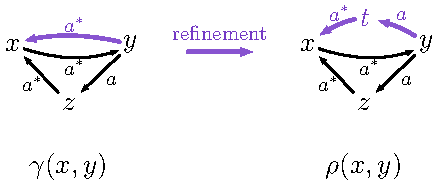
\includegraphics[width=\linewidth]{basic-refinement.pdf}
% 	\caption{\AP\label{fig:basic-refinement}A "refinement".}
% \end{marginfigure}
	
% \begin{marginfigure}
% 	\centering
% 	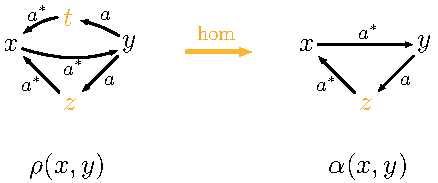
\includegraphics[width=\linewidth]{basic-hom.pdf}
% 	\caption{\AP\label{fig:basic-hom}A "strong onto homomorphism".}
% \end{marginfigure}

% \begin{definition}
%     \AP\label{def:atom-contraction}
%     \AP Given an "atom refinement" $\rho = x \atom{L_1} t_1 \atom{L_2} \hdots \atom{L_{n-1}} t_{n-1} \atom{L_n} y$ of $\gamma = x \atom{L} y$ as in \eqref{eq:refinement}, define
%     a ""condensation"" of $\rho$ between $t_i$ and $t_j$, where $0 \leq i,j \leq n$ and $j > i+1$, as any "C2RPQ" of the form:
%     \[
%         \rho' = x \atom{L_1} t_1 \atom{L_2} \hdots \atom{L_i} \textcolor{cPurple}{t_i \atom{K} t_j} \atom{L_{j+1}} \hdots
%         \atom{L_{n-1}} t_{n-1} \atom{L_n} y
%     \]
%     such that $\textcolor{cPurple}{K = \+A[q_i,q_j]}$.
% 	\begin{fact}
% 		\AP\label{fact:refinement-contained}
% 		Every "condensation" $\rho'$ of $\rho$ is a "refinement" of $\gamma$, and $\rho \contained \rho' \contained \gamma$.
% 	\end{fact}
%     \AP Informally, we will abuse the notation and
%     write $\intro*\contract{L_{i}\cdots L_{j}}$ to denote the language $K$---even if this language
%     does not only depend on $L_{i}\cdots L_{j}$.
% \end{definition}

% \begin{example}
%     \AP\label{ex:atom-refinement-twoway}
%     Let $\gamma(x,y) = x \atom{(aa^-)^*} y$ be a "C2RPQ" "atom", where
%     $(aa^-)^*$ is implicitly represented by its minimal automaton.
%     Then $\rho(x,y)$ is a "refinement" of "refinement length" seven of $\gamma(x,y)$
%     and $\rho'(x,y)$ is a "condensation" of $\rho(x,y)$, where:
%     \begin{align*}
%         \rho(x,y) & = x \atom{a} t_1 \atom{(a^-a)^*} t_2 \atom{(a^-a)^*} t_3
%             \coatom{a} t_4 \atom{(aa^-)^*} t_5 \atom{(aa^-)^*a} t_6 \coatom{a} y, \\
%         \rho'(x,y) & = x \atom{a} t_1 \atom{(a^-a)^*} t_2 \atom{(a^-a)^*} t_3
% 		\coatom{a} t_4 \atom{(aa^-)^*} y. 
%     \end{align*}
%     On the other hand, $\rho''(x,y) = x \atom{a} t_1 \coatom{a} y$ is not
%     a "condensation" of $\rho(x,y)$.
% \end{example}

% Given a natural number $m$, an \AP""$m$-refinement"" of a "C2RPQ" $\gamma(\bar x) = \bigwedge_{i} x_i \atom{L_i} y_i$ is any query resulting from: 1) replacing every "atom" by one of its "$m$-refinements@@atom", and 2)
% should some "$m$-refinements@@atom" have "equality atoms",
% collapsing the variables.
% \AP A ""refinement"" is an "$m$-refinement" for some $m$.
% Note that any "atom $m$-refinements" is, by definition, also an
% "atom $m'$-refinements" when $m \leq m'$: as a consequence, in the "refinement" of a "C2RPQ"
% the "atom refinements" need not have the same length.
% For instance, both $\rho(x,x) = x \atom{c} x$ and $\rho'(x,y) = x \atom{a} t_1 \atom{a} y \coatom{c} y$ are "refinements" of $\gamma(x,y) = x \atom{a^*} y \coatom{c} x$.

% %%%%%%%%%%%%%%%%%%%%%
% %     We will assume that a query "refinement" does not contain atoms with the language $\set{\epsilon}$; these are eliminated by identifying variables in a standard way. For example, if the result of replacing atoms by "atom refinements" yields $\gamma(x,z) = x \atom{\set{\epsilon}} y \land y \atom{\set{\epsilon}} z \land z \atom{a^*} x$ the associated "refinement" is then $\gamma(x,x) =  x \atom{a^*} x$.
% % \sidediego{CHECK}
% %%%%%%%%%%%%%%%%%%%%%
% For a given "C2RPQ" $\gamma$, let $\AP\intro*\Refin[\leq m](\gamma)$ be the set of all "$m$-refinements" of $\gamma$, and $\reintro*\Refin(\gamma)$ be the set of all its "refinements".
% Given a "refinement" $\rho(\bar x)$ of $\gamma(\bar x)$,
% its ""refinement length"" is the least natural number
% $m$ such that $\rho(\bar x) \in \Refin[\leq m](\gamma)$.
% Note that if the automaton representing a language $L$ has more than one final state, for instance the minimal automaton for $L = a^+ + b^+$,
% then $x \atom{L} y$ is not a "refinement" of itself.
% However, it will always be "equivalent" to a union of refinements: in
% this example, $x \atom{a^+ + b^+} y$ is "equivalent" to the union of
% $x \atom{a^+} y$ and $x \atom{b^+} y$, which are both "refinements"
% of the original "C2RPQ".

% \paragraph*{Expansions}
% %%%%%%%%%%%%%%%%%%%%%
% % \sidediego{CHECK}
% % Observe that a "C2RPQ" $\gamma$ whose every language is of the form $\set{z}$ for $z \in \Aext \dcup \set{\varepsilon}$ is equivalent to a "conjunctive query" $\tilde \gamma$. For example, $\gamma(x,y) = x \atom{\varepsilon} y \land y \atom{\set{a^-}} z$ is equivalent to $\tilde\gamma(y,y) = z \atom{a} y$. 
% Remember that a "C2RPQ" whose languages are
% of the form $\set{a}$ or $\set{a^-}$ for $a \in \A$ is in effect a "CQ".
% The \AP""expansions"" of a "C2RPQ" $\gamma$ is the set $\intro*\Exp(\gamma)$ of all "CQs" which are "refinements" of $\gamma$.
% In other words, an "expansion" of $\gamma$ is any "CQ" obtained from $\gamma$
% by replacing each "atom" $x \atom{L} y$ by a path $x \atom{w} y$ for some
% word $w \in L$.
% For instance, $\xi(x,y) = x \atom{a} t_1 \coatom{a} t_2 \atom{a} t_3 \coatom{a} y$
% is an "expansion" of $\rho(x,y) = x \atom{(aa^-)^*} y$.
% %%%%%%%%%%%%%%%%%%%%%
% % l228: But, isn't this the notation used on all previous pages?
% % We will henceforth identify a "C2RPQ" atom $x \atom{\set{a}} y$ \resp{$x \atom{\set{a^-}} y$} as simply $x \atom{a} y$ \resp{$x \coatom{a} y$}, and thus we will consider that the class of "CQs" is a syntactic fragment of the class of "C2RPQs".

% Any "C2RPQ" is equivalent to the infinitary union of its "expansions". In light of this, the semantics for "UC2RPQ" can be rephrased as follows. 
% Given a "UC2RPQ" $\Gamma(\bar x)$ and a graph database $G$, 
% the "evaluation" of $\Gamma(\bar x)$ over $G$, denoted by $\Gamma(G)$, is the set of tuples 
% $\bar{v}$ of nodes for which there is $\anexpansion \in \Exp(\Gamma)$ such that there is a "homomorphism" $\anexpansion \homto G$ that sends $\bar x$ onto $\bar v$.  
% Similarly, "containment" of "UC2RPQs" can also be characterized in terms of expansions.

% \begin{proposition}[Folklore, see e.g. {\cite[Proposition 3.2]{FlorescuLevySuciu1998Containment}} or
%     {\cite[Theorem 2]{CalvaneseDeGiacomoLenzeriniVardi2000Containment}}]
%     \AP\label{prop:cont-char-exp-st} 
%     Let $\Gamma_1$ and $\Gamma_2$ be "UC2RPQs". Then the following are equivalent
%     \begin{itemize}
%         \item $\Gamma_1 \contained \Gamma_2$;
%         \item for every $\anexpansion_1\in \Exp(\Gamma_1)$, $\anexpansion_1 \contained \Gamma_2$;
%         \item for every $\anexpansion_1\in \Exp(\Gamma_1)$ there is $\anexpansion_2\in \Exp(\Gamma_2)$ such that $\anexpansion_2\homto \anexpansion_1$. 
%     \end{itemize}
% \end{proposition}

% Note that since an "expansion" of $\gamma$ is also a "refinement" of $\gamma$, it also
% holds that $\gamma$ is "semantically equivalent" to the infinitary union of its "refinements".

% \AP Given a "C2RPQ" $\gamma$, an \AP""internal path"" is a sequence of atoms\footnote{We write
% $x \symatom{\lambda} y$ to mean that there is either an "atom" $x \atom{\lambda} y$
% \textbf{or} an "atom" $x \coatom{\lambda} y$.}
% \[
% 	x_0 \symatom{L_1} x_1 \symatom{L_2} \cdots \symatom{L_{n-1}} x_{n-1} \symatom{L_n} x_n
% \]
% where each $x_i$ for $i \in \lBrack 1,n-1 \rBrack$ has total degree
% exactly 2 and is existentially quantified.
% \AP Its ""contraction@@path"" is defined as the edge
% \[
% 	x_0 \atom{K_1 \cdot K_2 \cdots K_{n-1} \cdot K_n} x_n,
% \]
% where $K_i \defeq L_i$ if the "atom" between $x_i$ and $x_{i+1}$ is directed from
% left to right, and $K_i \defeq L_i^{-}$ if the "atom" is directed from right to left.\footnote{Given a regular language $L$ over $\Aext$, we define a regular language $L^-$ over $\Aext$ by induction on regular expressions: $\emptyset^- \defeq \emptyset$, $(a)^- \defeq a^-$, $(a^-)^- \defeq a$, $(L_1\cdot L_2)^- \defeq L_2^- \cdot L_1^-$, $(L^*)^- \defeq (L^-)^*$ and $(L_1 + L_2)^- \defeq L_1^- + L_2^-$. Then, for any graph, there is a path from $x$ to $y$ labelled by
% a word of $L$ "iff" there is a path from $y$ to $x$ labelled by a word of $L^-$.}

% \AP Similarly, a ""one-way internal path"" is a sequence of atoms 
% \[
% 	x_0 \atom{L_1} x_1 \atom{L_2} \cdots \atom{L_{n-1}} x_{n-1} \atom{L_n} x_n
% \]
% where each $x_i$ for $i \in \lBrack 1,n-1 \rBrack$ has exactly in-degree
% and out-degree 1 in $\gamma$ and is existentially quantified.
% \AP Its ""one-way contraction@@path"" is defined as the edge
% \[
% 	x_0 \atom{L_1 \cdot L_2 \cdots L_{n-1} \cdot L_n} x_n.
% \]

% \AP A ""contraction"" (resp.\ ""one-way contraction"") of a "C2RPQ" is any query obtained
% by iteratively replacing some "internal paths" (resp.\ "one-way internal paths") by
% their "contraction@@path" (resp.\ "one-way contraction@@path"). By definition,
% a query is always "equivalent" to any of its "contractions" or "one-way contractions".